\begin{figure}[t]
    \centering
     \begin{subfigure}{0.358\textwidth}
        \centering
        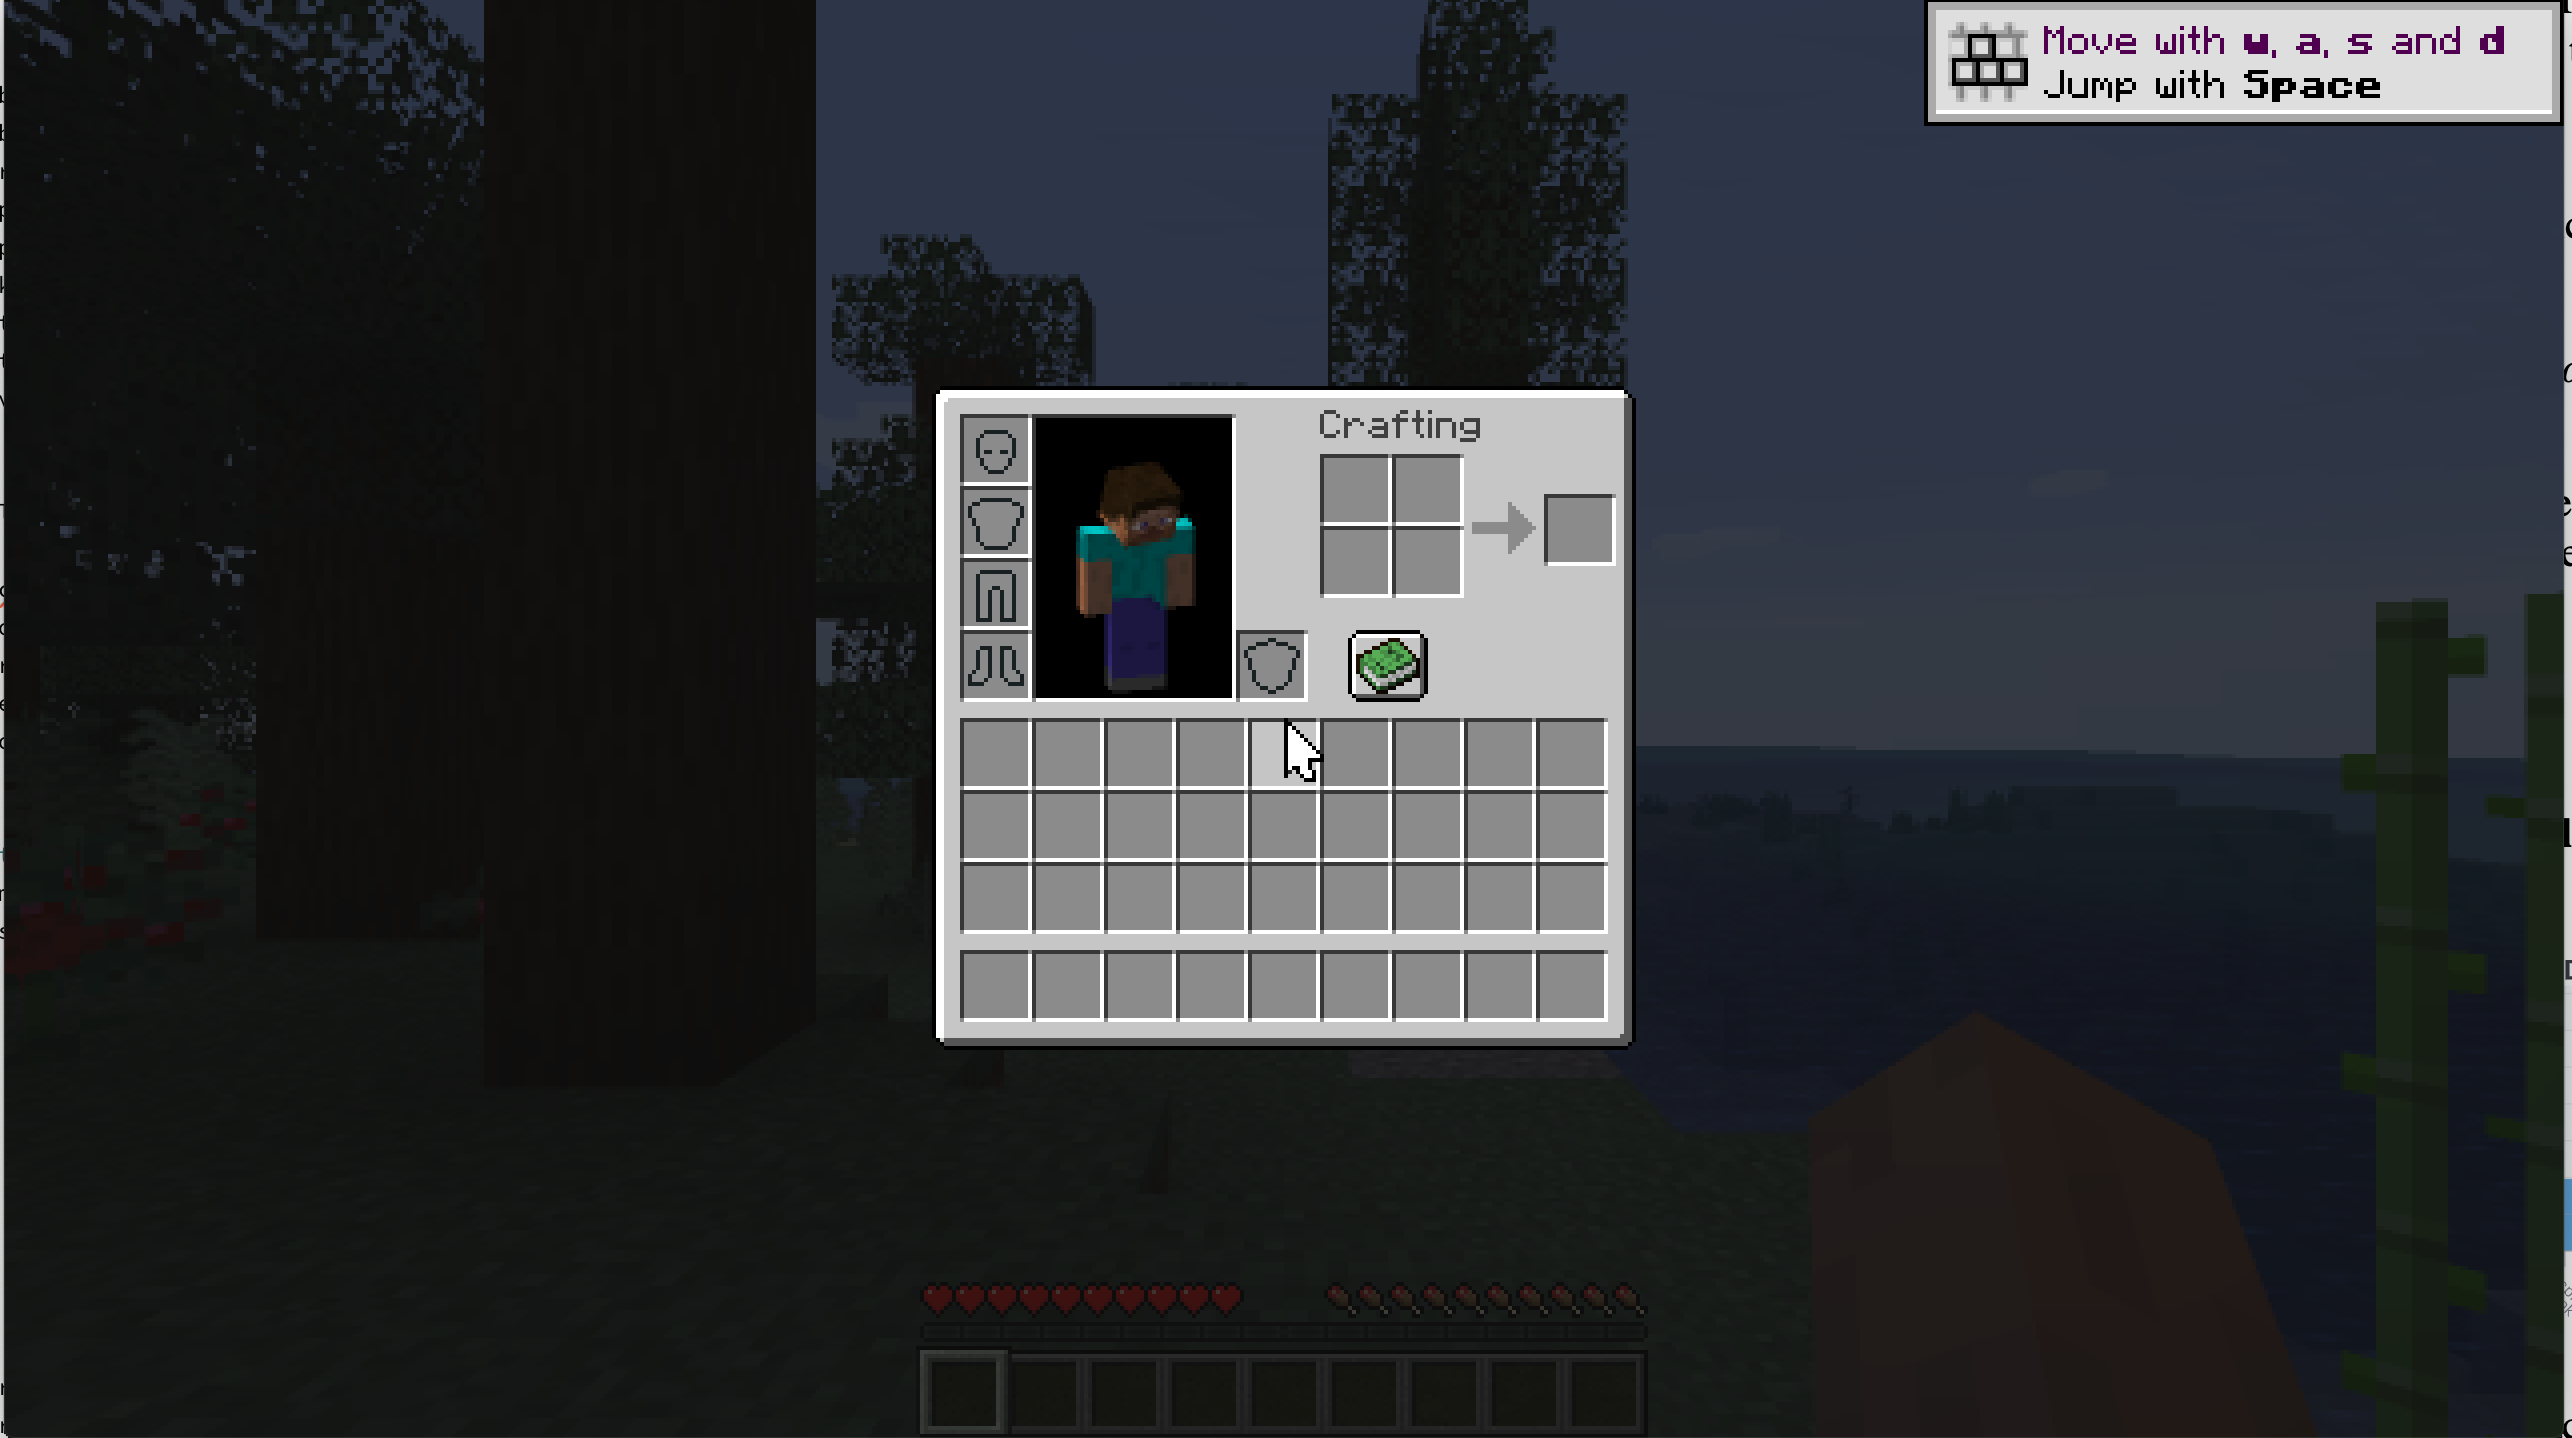
\includegraphics[width=\linewidth]{assets/a_1/mc_gameplay_640x360_gui.png} 
    \end{subfigure}
    \begin{subfigure}{0.2\textwidth}
        \centering
        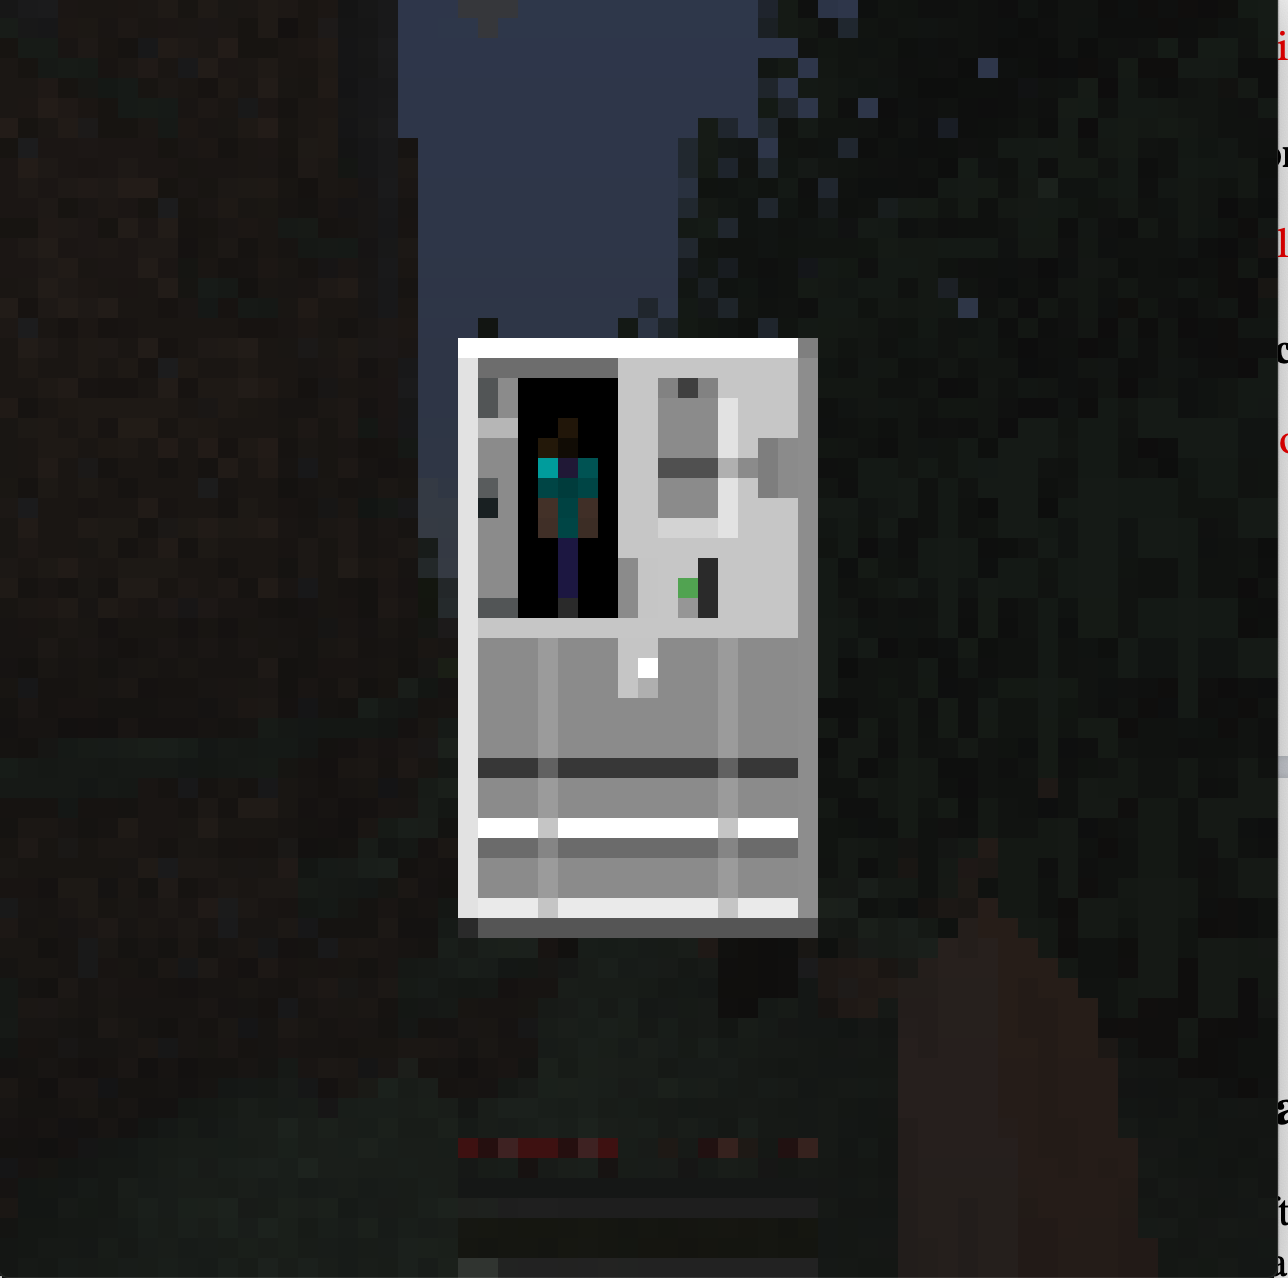
\includegraphics[width=\linewidth]{assets/a_1/mc_gameplay_128x128_gui.png} 
    \end{subfigure}
    \begin{subfigure}{0.2\textwidth}
        \centering
        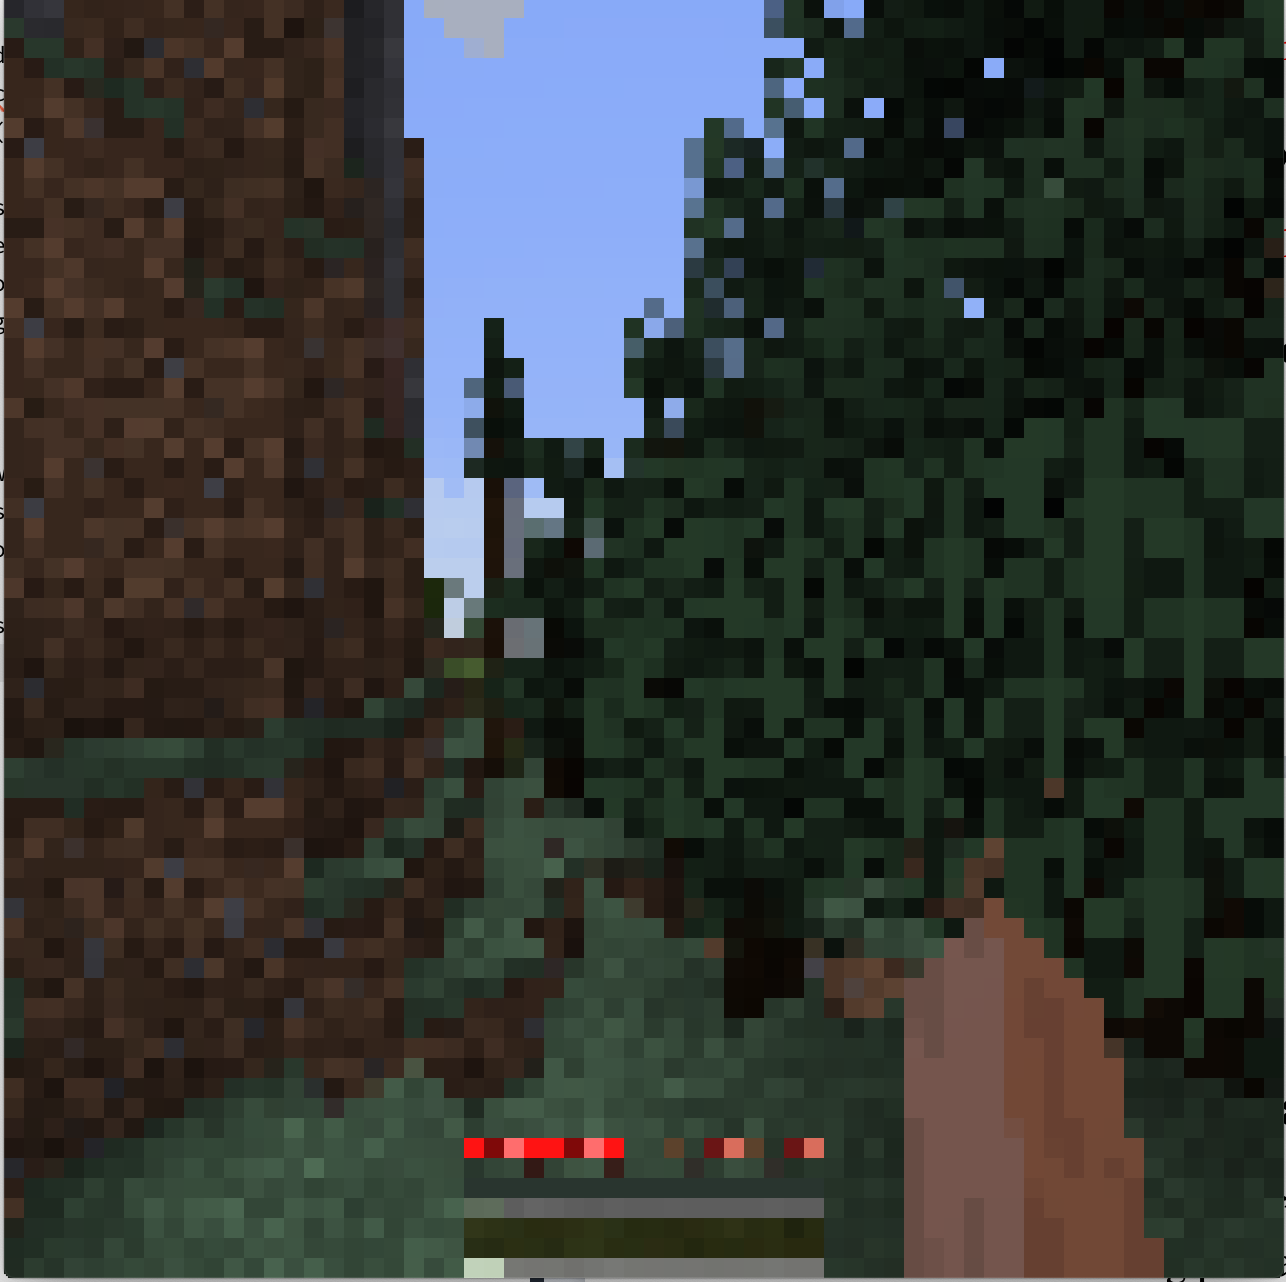
\includegraphics[width=\linewidth]{assets/a_1/mc_gameplay_128x128.png} 
    \end{subfigure}
    \caption{\label{fig:a_1_observations}\textbf{(Left)} Sample of a Minecraft frame in the original resolution (640x360) with an in-game GUI open. The mouse cursor can be seen in the center of the image. This particular GUI shows the player's inventory and can be used to craft very basic items. \textbf{(Middle)} We downsample images to 128x128 for computational reasons. Shown is a downsampled observation with an in-game GUI for crafting. This is the resolution used by our models. \textbf{(Right)} A 128x128 observation as seen by our models without in-game GUI. The health, hunger, hotbar overlays, and agent hand can be seen in the lower part of the image.}
\end{figure}
\section{Minecraft environment details}
\label{appendix:minecraft_environment}

Our Minecraft training environment is a hybrid between MineRL \cite{guss2019minerl} and the MCP-Reborn (\href{https://github.com/Hexeption/MCP-Reborn}{github.com/Hexeption/MCP-Reborn}) Minecraft modding package. Unlike the regular Minecraft game, in which the server (or the "world") always runs at 20Hz and the client runs as fast as rendering can complete (typically at 60-100Hz), in our version the client and server run in the same thread at the same frequency. This allows us to run the environment slower or faster than real time, while avoiding artifacts like missing chunks of the world. The action and observation spaces are similar to those of MineRL environments and are described in more detail in the following subsections. The environment also returns diagnostic information, such as in-game stats, contents of the agent's inventory, whether any in-game GUI is open, etc., which we use for tracking and recording but not as inputs to the models. The episode length is 10 minutes for RL experiments and 60 minutes for BC model evaluations. The agent can "die" in a number of ways, such as staying under water for too long and drowning, being killed by hostile mobs, or falling from a tall structure. We do not terminate the episode on agent "death". Instead, just as for humans in the regular Minecraft game, the agent drops all its items when it dies and respawns at a random spot close to the initial spawning spot in the same Minecraft world. The policy state is not masked on death, so the model can remember the fact that it has died and act accordingly.

\subsection{Observation space}
\label{appendix:minecraft_env_observation_space}
The  environment observations are simply the raw pixels from the Minecraft game that a human would see. Unlike MineRL, we do not remove overlays like the hotbar, health indicators, and the animation of a moving hand shown in response to the attack or ``use'' actions. The field of view is 70 degrees, which corresponds to the Minecraft default. GUI scale (a parameter controlling the size of the in-game GUI) is set to 2, and brightness is set to 2 (which is not a Minecraft default, but is very frequently used in online videos).  The rendering resolution is 640x360, which is downsampled to 128x128 before being input to the models. We empirically found 128x128 to be the smallest resolution for which in-game GUI elements are still discernible, and then chose that to minimize compute costs. Whenever an in-game GUI is open, we additionally render an image of a mouse cursor at the appropriate mouse position to match what a human player's operating system does (Fig. \ref{fig:a_1_observations}).

\subsection{Action space}
\label{appendix:action_space}
Our action space includes almost all actions directly available to human players, such as keypresses, mouse movements, and clicks. The specific binary actions we include are shown in Table~\ref{table:binary_actions}.

\begin{table}[htpb]
\begin{center}
\renewcommand\arraystretch{1.4}
\begin{tabular}{ |c|c|p{0.55\linewidth}| } 
\hline
 \textbf{Action} & \textbf{Human action} & \textbf{Description}\\ 
 \hline
 \texttt{forward} & W key & Move forward. \\
 
 \texttt{back} & S key & Move backward.\\ 
 
 \texttt{left} & A key & Strafe left. \\ 
 
 \texttt{right} & D key & Strafe right.\\
 
 \texttt{jump} & space key & Jump.\\
 
 \texttt{inventory} & E key & Open or close inventory and the 2x2 crafting grid. \\
 
 \texttt{sneak} & shift key & Move carefully in current direction of motion. In the GUI it acts as a modifier key: when used with \texttt{attack} it moves item from/to the inventory to/from the hotbar, and when used with \texttt{craft} it crafts the maximum number of items possible instead of just 1.\\
 
 \texttt{sprint} & ctrl key & Move fast in the current direction of motion. \\
 
 \texttt{attack} & left mouse button & Attack; In GUI, pick up the stack of items or place the stack of items in a GUI cell; when used as a double click (attack - no attack - attack sequence), collect all items of the same kind present in inventory as a single stack.\\
 
 \texttt{use} & right mouse button & Place the item currently held or use the block the player is looking at. In GUI, pick up the stack of items or place a single item from a stack held by mouse. \\
 
 \texttt{drop} & Q key & Drop a single item from the stack of items the player is currently holding. If the player presses ctrl-Q then it drops the entire stack. In the GUI, the same thing happens except to the item the mouse is hovering over. \\
 
 \texttt{hotbar.[1-9]} & keys 1 -- 9 & Switch active item to the one in a given hotbar cell. \\
\hline
\end{tabular}
\end{center}
\caption{\label{table:binary_actions}Binary actions included in the action space. \url{https://minecraft.fandom.com/wiki/Controls} has more detailed descriptions of each action.}
\end{table}

One difference between the human action space and our agent's is that we disallow typing arbitrary letters, which is only useful for entering text into the search bar of the crafting recipe book. Humans can either do that or browse the recipe book with the mouse, the latter of which our agent can still do. However, because we do allow the agent to press letters that are also shortcuts for actions (e.g.\ outside of the GUI, the "W" key triggers the \texttt{forward} action) agents are able to press a few keys within the GUI (W, A, S, D, E, Q) that produce letters if the recipe book search bar is selected. We have not seen agents attempt to search the recipe book with these letters. Instead, our agents navigate the recipe book with the mouse or craft by dragging items around the crafting window. 

In addition to the binary (on/off) keypress actions, our action space also includes mouse movements. As with human gameplay, when in-game GUIs are not open, mouse X and Y actions change the agent's yaw and pitch, respectively. When a GUI is open, camera actions move the mouse cursor. Mouse movements are relative (i.e. they move the mouse or camera relative to the current position, and thus their effect depends on the current position).

Inventory interaction in Minecraft requires fine-grained mouse movements to achieve tasks such as crafting and smelting, while mining and navigating the world can be achieved with coarser mouse action. To be able to achieve both with the same action space, we implemented mouse movements as a set of discrete actions with foveated binning along each axis (Fig. \ref{fig:a_1_camera_binning}), which in preliminary experiments we found to improve crafting performance.

\begin{figure}[htbp]
\begin{center}
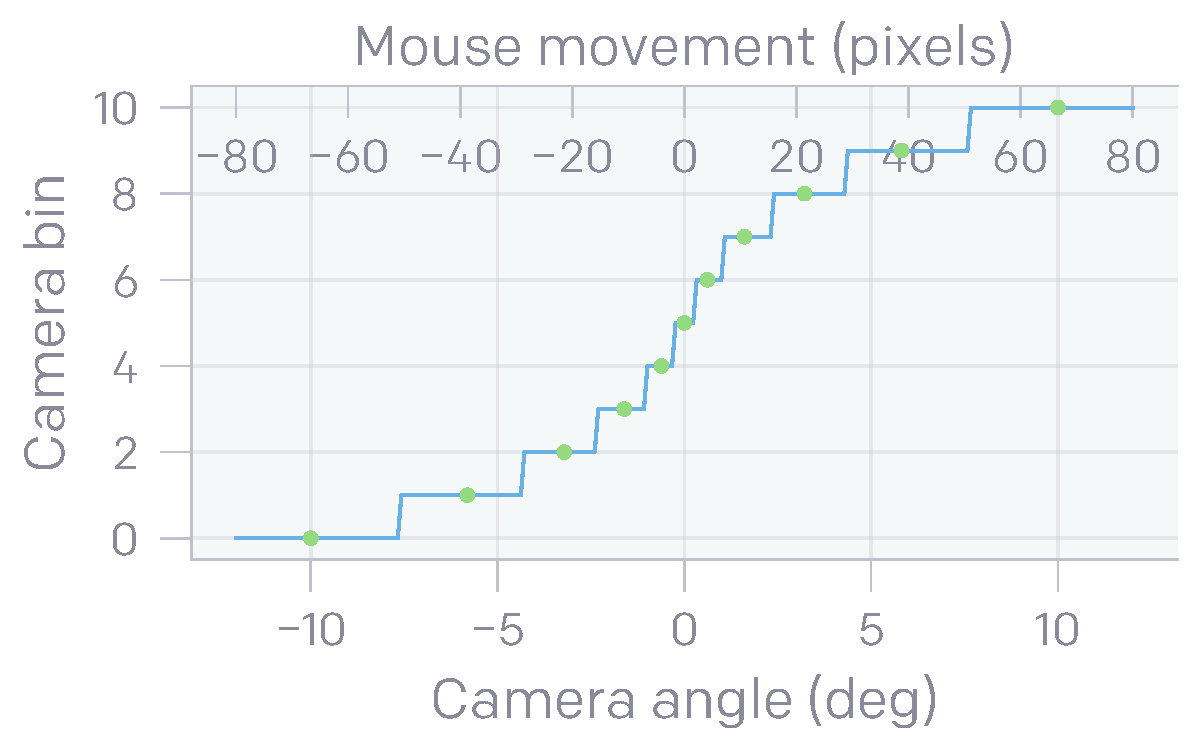
\includegraphics[width=0.5\linewidth]{assets/a_1/camera_bins.pdf}
\end{center}
\vspace{-8px}
\caption{\label{fig:a_1_camera_binning} Relative camera angle or mouse movement in pixels vs.\ action bin. The same binning is used for both X and Y coordinates. The binning is foveated, meaning that binning is more fine-grained for smaller movements and more coarse-grained for larger movements. There are 11 bins for each axis (X and Y). The center of each bin (indicated with green circles) is used when un-discretizing movements (that is, when converting from an action expressed as a bin to a camera angle or mouse movement).}
\end{figure}
